\chapter{Introducción}

\section{Contextualización}

\subsection{Nivel Macro}
La desnutrición crónica se mide como retraso en el crecimiento en talla para la edad y afecta a millones de niños menores de cinco años en el mundo. Una revisión sobre diagnóstico de malnutrición en preescolares estima cerca de 149 millones de niños con este problema y lo asocia con aproximadamente el 45\,\% de las muertes infantiles \cite{shindediagnosing}. Sus consecuencias incluyen deterioro del desarrollo cognitivo, menor rendimiento escolar y mayor riesgo de enfermedades crónicas en la edad adulta \cite{nu17101642}. Por ello, la reducción de la malnutrición infantil forma parte de los Objetivos de Desarrollo Sostenible 2 y 3 \cite{11355002}.

En los últimos años se ha explorado el aprendizaje automático (\textit{Machine Learning}, ML) para clasificar el estado nutricional infantil a partir de encuestas de salud. Un metaanálisis de 11 estudios con datos de las Encuestas Demográficas y de Salud (DHS) reportó una exactitud agrupada de \SI{68.92}{\percent} para el retraso en talla, con heterogeneidad muy alta entre estudios \cite{ijerph22030449}. Este resultado muestra que el desempeño depende de los datos y del protocolo empleados, y no solo del algoritmo.

\subsection{Nivel Meso}
En Ecuador, la prevalencia de desnutrición crónica en niños menores de dos años fue de \SI{19.3}{\percent} según el panel de indicadores del INEC basado en la ENSANUT 2018, con valores más altos en población indígena (\SI{32.3}{\percent}), en el área rural (\SI{22.1}{\percent}) y en el primer quintil de ingresos (\SI{21.8}{\percent}) (Figura~\ref{fig:inec}). Una revisión sistemática de 17 estudios con cerca de \num{12000} niños ecuatorianos de 1 a 11 años ubica la desnutrición crónica entre \SI{15}{\percent} y \SI{35}{\percent}, y señala la educación materna y el nivel socioeconómico como determinantes principales \cite{nu17223608}. La Encuesta Nacional sobre Desnutrición Infantil (ENDI) 2023--2024 registró \SI{18.7}{\percent} de retraso en talla en niños de 0 a 23 meses \cite{nu18142232}.

\begin{figure}[H]
  \centering
  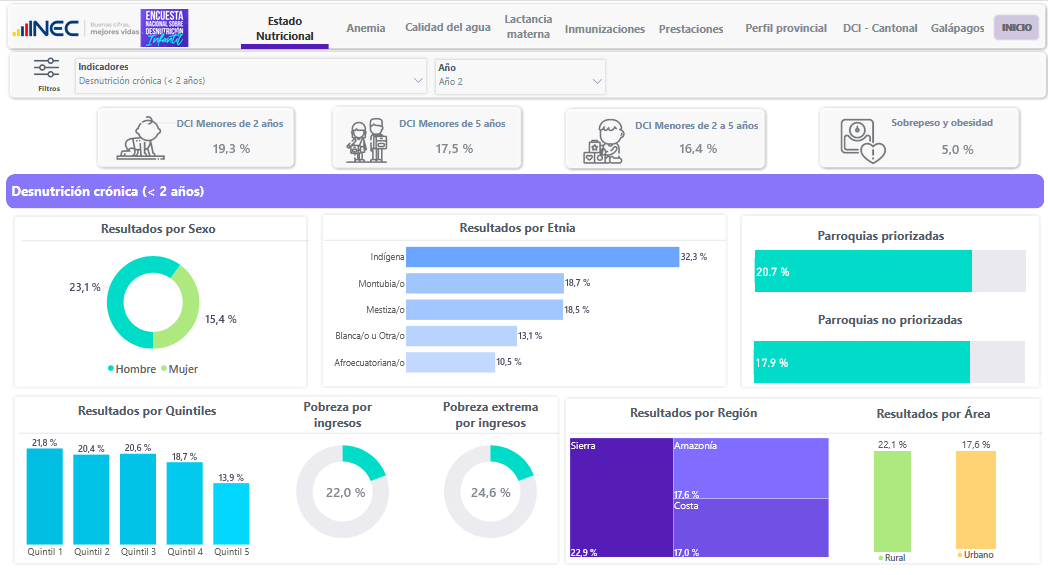
\includegraphics[width=0.85\textwidth]{figuras/inec-estado-nutricional.png}
  \caption{Panel de indicadores de desnutrición crónica en menores de 2 años. Fuente: INEC, ENSANUT 2018 \cite{inec2018ensanut}.}
  \label{fig:inec}
\end{figure}

\subsection{Nivel Micro}
Este trabajo no se desarrolló para una entidad receptora específica: es un prototipo académico de la Universidad Tecnológica Indoamérica que utiliza microdatos públicos de la ENSANUT 2018. La provincia de Tungurahua se toma como territorio de análisis por su combinación de áreas urbanas y rurales. En la base de modelado de este trabajo (niños de 0 a 59 meses; \num{18493} registros), \num{531} corresponden a Tungurahua, con una prevalencia muestral de \SI{30.9}{\percent} frente a \SI{24.7}{\percent} en el conjunto nacional de la misma base (Figura~\ref{fig:prevalencia}). Estas cifras son muestrales, no están ponderadas por el diseño de la encuesta y no son comparables con las estimaciones poblacionales del INEC, que corresponden a otra población de referencia (menores de dos años).

\begin{figure}[H]
  \centering
  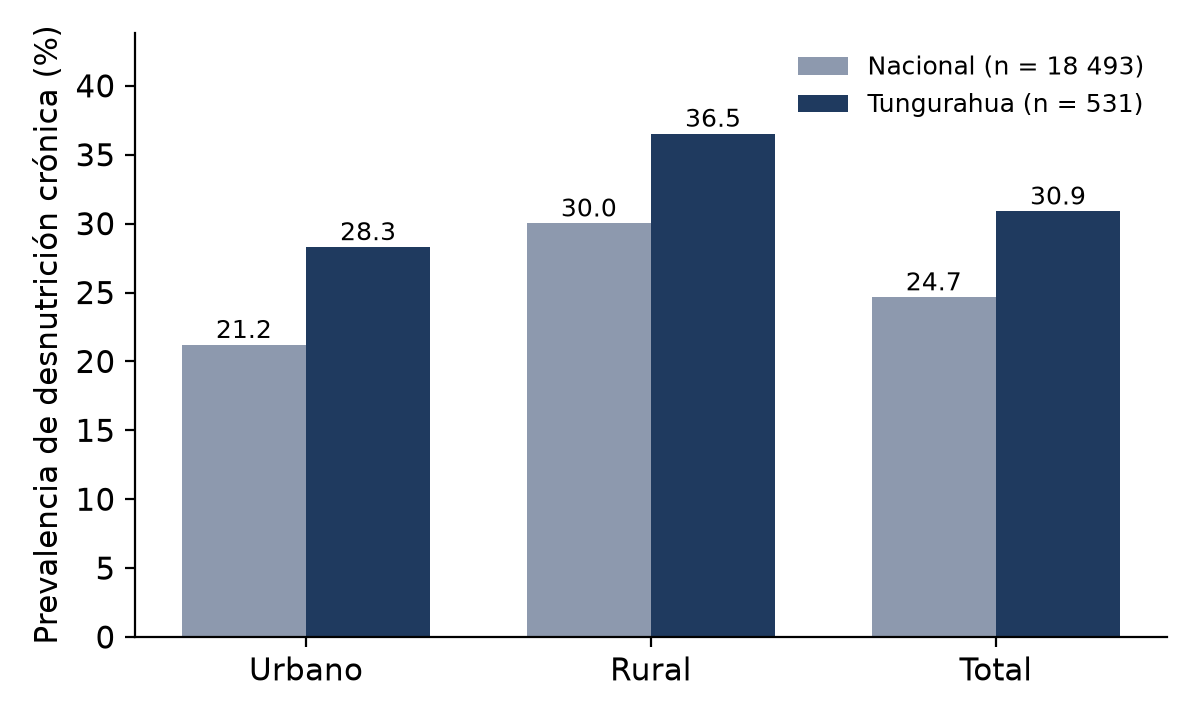
\includegraphics[width=0.75\textwidth]{figuras/prevalencia-area.png}
  \caption{Prevalencia muestral de desnutrición crónica por área de residencia: base nacional y subconjunto de Tungurahua. Elaboración propia a partir de la ENSANUT 2018 (sin ponderar).}
  \label{fig:prevalencia}
\end{figure}

\section{Estado del Arte}
\subsection{Protocolo de búsqueda}
La revisión se limitó a estudios que aplican ML a la clasificación del estado nutricional infantil o que describen el contexto nutricional de Ecuador. Se consultaron IEEE Xplore, ScienceDirect, MDPI, PubMed y Google Académico con combinaciones de los términos \textit{child malnutrition}, \textit{stunting}, \textit{machine learning}, \textit{ENSANUT} y \textit{Ecuador}. Se incluyeron artículos de 2019 a 2026 en español o inglés con texto completo disponible y se excluyeron los que no reportaban población, método o métricas. Se analizaron 10 trabajos, resumidos en la Tabla~\ref{tab:estado-arte}.

\begingroup
\footnotesize\setlength{\tabcolsep}{4pt}\arrayrulecolor{black!55}\renewcommand{\arraystretch}{1.15}
\begin{longtable}{|p{1.1cm}|p{2.7cm}|p{2.9cm}|p{2.7cm}|p{2.7cm}|}
  \caption{Comparación de los trabajos revisados con la presente tesis.}
  \label{tab:estado-arte}\\ \hline
  \enc{Estudio} & \enc{Datos y población} & \enc{Métodos y métricas} & \enc{Resultados y limitaciones} & \enc{Relación con la tesis}\\ \hline
  \endfirsthead
  \tablacont{5}\hline
  \enc{Estudio} & \enc{Datos y población} & \enc{Métodos y métricas} & \enc{Resultados y limitaciones} & \enc{Relación con la tesis}\\ \hline
  \endhead
  \hline\endfoot
  \cite{nu18142232} & ENDI 2023--2024 (Ecuador); \num{8344} niños de 0 a 23 meses; retraso en talla \SI{18.7}{\percent} & Modelos de ensamble con explicabilidad (SHAP); exactitud, ROC-AUC, precisión, F1, sensibilidad, especificidad y Brier en un conjunto de prueba & AUC de 0.62 a 0.66 (desempeño modesto a moderado); diseño transversal; SHAP no implica causalidad & Referente más cercano (mismo país e indicador). Sus AUC delimitan el rango esperable.\\ \hline
  \cite{ijerph22030449} & Metaanálisis de 11 estudios (de 789) con datos DHS; niños menores de 5 años & RF, gradient boosting, SVM, k-NN y regresión logística; riesgo de sesgo con PROBAST & Exactitud agrupada: \SI{68.92}{\percent} (talla), \SI{84.39}{\percent} (emaciación), \SI{73.60}{\percent} (bajo peso); $I^2$ = \SI{100}{\percent} & Da el nivel de referencia de exactitud y justifica reportar métricas por clase.\\ \hline
  \cite{Indrisari_Febiansyah_Adiwinoto_2025} & Revisión sistemática de 20 artículos (2020--2024) sobre retraso en talla en Indonesia & RF, SVM y redes neuronales; exactitud de \SI{72}{\percent} a \SI{99.92}{\percent} & Desbalance de clases, baja interpretabilidad y falta de validación externa & Justifica tratar el desbalance y declarar la ausencia de validación externa.\\ \hline
  \cite{11355002} & Revisión sistemática sobre predicción de retraso en talla (ODS 2 y 3) & Árboles de decisión, RF, redes neuronales y SVM & Resultados variables según calidad de los datos y metodología & Justifica comparar varios algoritmos con el mismo protocolo.\\ \hline
  \cite{11042152} & Estudio analítico de modelos; encuestas IDHS, BDHS y MICS & Árboles, SVM, RF, XGBoost y redes; comparación de metodologías & Falta de métricas estandarizadas y limitada generalización & Respalda la definición explícita de métricas y de partición.\\ \hline
  \cite{JANSSEN2024100264} & Revisión sistemática de IA en malnutrición (niños y adultos) & Predomina el aprendizaje supervisado & Más del \SI{90}{\percent} de los modelos no se usa en la práctica & Motiva declarar el alcance de prototipo académico.\\ \hline
  \cite{KIRK20222573} & Revisión sobre ML en investigación nutricional & Marco de trabajo; validación cruzada frente a partición simple & Riesgo de sobreajuste sin validación sólida & Sustenta la validación cruzada y el reporte del sobreajuste.\\ \hline
  \cite{ijerph23020240} & \num{303} recicladores de tres ciudades de Ecuador; adultos & RF, CatBoost y XGBoost; SMOTE solo en entrenamiento; ROC-AUC y sensibilidad por clase & Diseño transversal y tamaño muestral limitado & Ejemplo de manejo de desbalance sin fuga; población distinta.\\ \hline
  \cite{diagnostics16142147} & Datos demográficos del Hospital Isidro Ayora (Quito); preeclampsia & Seis modelos; F1 y SHAP; se añadió un conjunto sintético & F1 de 0.80 y AUC de 0.94 a 0.96; escasez de variables clínicas & Otro evento de salud en Ecuador; contexto del uso de ML con datos nacionales.\\ \hline
  \cite{nu17223608} & Revisión sistemática PRISMA de 17 estudios; cerca de \num{12000} niños ecuatorianos & Sin modelos de ML; síntesis de prevalencias y determinantes & Desnutrición crónica de \SI{15}{\percent} a \SI{35}{\percent}; mayor en zonas rurales e indígenas & Fundamenta las variables sociodemográficas y el contexto ecuatoriano.\\ \hline
\end{longtable}
\endgroup

\subsection{Criterios de selección y documentos excluidos}
La Tabla~\ref{tab:criterios} resume los criterios aplicados. La revisión se hizo sobre 15 documentos disponibles a texto completo; 10 cumplieron los criterios y se incluyeron en la Tabla~\ref{tab:estado-arte}. La Figura~\ref{fig:seleccion} muestra el flujo y la Tabla~\ref{tab:excluidos} los motivos de exclusión. No se registró el número de resultados devueltos por cada base de búsqueda, por lo que el flujo parte de los documentos ya reunidos y no constituye una revisión sistemática formal.

\begin{table}[H]
  \caption{Criterios de inclusión y exclusión.}
  \label{tab:criterios}
  \tablabase\small
  \begin{tabular}{|p{2.6cm}|p{5.6cm}|p{5.4cm}|}
    \hline
    \enc{Aspecto} & \enc{Inclusión} & \enc{Exclusión}\\ \hline
    Tema & Aplicación de ML a estado nutricional infantil, o contexto nutricional de Ecuador & Evaluación nutricional sin ML; temas ajenos a nutrición infantil\\ \hline
    Periodo & Publicaciones de 2019 a 2026 & Anteriores a 2019\\ \hline
    Idioma y acceso & Español o inglés; texto completo disponible & Sin texto completo\\ \hline
    Contenido mínimo & Población o fuente de datos, método y algún resultado o limitación & No reporta población, método o resultados\\ \hline
  \end{tabular}
\end{table}

\begin{figure}[H]
  \centering
  \begin{tikzpicture}[font=\footnotesize, node distance=6mm,
    caja/.style={draw=black!60, rounded corners=2pt, align=center, text width=4.4cm, minimum height=1.3cm, fill=white},
    flecha/.style={-{Stealth[length=2mm]}, black!60}]
    \node[caja] (a) {\textbf{Documentos reunidos}\\ 15 a texto completo};
    \node[caja, right=12mm of a] (b) {\textbf{Incluidos}\\ 10 en la Tabla~\ref{tab:estado-arte}};
    \node[caja, below=8mm of b] (c) {\textbf{Excluidos}\\ 5, con motivo en la Tabla~\ref{tab:excluidos}};
    \draw[flecha] (a) -- (b); \draw[flecha] (a.south) |- (c.west);
  \end{tikzpicture}
  \caption{Flujo de selección de los documentos revisados. Elaboración propia.}
  \label{fig:seleccion}
\end{figure}

\begin{table}[H]
  \caption{Documentos no incluidos en la comparación y motivo.}
  \label{tab:excluidos}
  \tablabase\small
  \begin{tabular}{|p{4.9cm}|p{8.7cm}|}
    \hline
    \enc{Documento} & \enc{Motivo de exclusión}\\ \hline
    Revisión narrativa sobre el modelo ABCDEFG de evaluación nutricional \cite{app16020845} & Evaluación nutricional clínica sin modelos de ML\\ \hline
    Comparación de métodos de evaluación nutricional del recién nacido \cite{nu17101642} & Neonatos y métodos antropométricos, sin ML\\ \hline
    Efecto de la austeridad sobre los niños en países de ingresos bajos y medios \cite{DAOUD2024102973} & Objetivo económico y de inferencia causal, no de clasificación nutricional\\ \hline
    Minería de datos y ML en diagnóstico clínico \cite{Saberi-Karimian19052021} & Enfoque clínico general, sin población infantil ni indicador nutricional\\ \hline
    Diagnóstico de malnutrición en preescolares con ML \cite{shindediagnosing} & Revisión sin población, métricas ni limitaciones comparables; se usa solo como contexto\\ \hline
  \end{tabular}
\end{table}


\subsection{Síntesis y aporte de la tesis}
Los trabajos revisados muestran tres patrones. Primero, los algoritmos de árboles y de \textit{boosting} son los más usados, pero ninguno es superior en todos los conjuntos de datos \cite{11355002}. Segundo, el desempeño reportado depende de la métrica: la exactitud puede ser alta o engañosa cuando las clases están desbalanceadas, y el estudio más reciente con datos ecuatorianos reporta AUC modestos de 0.62 a 0.66 \cite{nu18142232}. Tercero, la mayoría de los estudios usa validación interna, y la falta de validación externa y de interpretabilidad son limitaciones recurrentes \cite{Indrisari_Febiansyah_Adiwinoto_2025,JANSSEN2024100264}.

Frente a ello, esta tesis aporta: (i) un protocolo con prevención documentada de fuga de información y reporte de métricas por clase, incluida PR-AUC; (ii) una evaluación separada para Tungurahua con intervalos de confianza; y (iii) un prototipo reproducible (API y tablero) con casos de prueba funcionales. No aporta validación externa ni validación clínica.

\section{Planteamiento del Problema}
Los microdatos de la ENSANUT 2018 se emplean sobre todo para estimar prevalencias. Aprovecharlos con ML exige resolver tres dificultades verificables en la base: 350 variables en \num{20510} registros con códigos numéricos y valores especiales; \num{2017} registros (\SI{9.8}{\percent}) sin la variable objetivo; y desbalance de clases cercano a 3 a 1. A esto se suma la escasa evidencia, para Tungurahua, de cuánto funciona un clasificador entrenado con datos nacionales. El problema central es, por tanto, la ausencia de un procedimiento reproducible que clasifique la desnutrición crónica infantil con métricas por clase y muestre su desempeño para Tungurahua (Figura~\ref{fig:arbol}).

\begin{figure}[H]
  \centering
  \begin{tikzpicture}[font=\footnotesize, node distance=6mm,
    caja/.style={draw=black!60, rounded corners=2pt, align=center, text width=4.1cm, inner sep=4pt, fill=white},
    central/.style={draw=black!80, thick, rounded corners=2pt, align=center, text width=11cm, inner sep=6pt, fill=black!6},
    flecha/.style={-{Stealth[length=2mm]}, black!60}]
    \node[caja] (e1) {Conclusiones basadas en exactitud global, poco informativa con clases desbalanceadas};
    \node[caja, right=3mm of e1] (e2) {Análisis manual, difícil de reproducir};
    \node[caja, right=3mm of e2] (e3) {Sin evidencia de desempeño para Tungurahua};
    \node[central, below=10mm of e2] (c) {\textbf{PROBLEMA CENTRAL}\\ Ausencia de un procedimiento reproducible que clasifique la desnutrición crónica infantil con métricas por clase y evalúe su desempeño en Tungurahua};
    \node[caja, below=10mm of c] (c2) {Datos fragmentados: 350 variables, valores especiales y códigos numéricos};
    \node[caja, left=3mm of c2] (c1) {\num{2017} registros (\SI{9.8}{\percent}) sin variable objetivo};
    \node[caja, right=3mm of c2] (c3) {Desbalance de clases (\SI{24.7}{\percent} de casos) y pocos registros de Tungurahua (531)};
    \foreach \n in {e1,e2,e3} \draw[flecha] (c.north) -- (\n.south);
    \foreach \n in {c1,c2,c3} \draw[flecha] (\n.north) -- (c.south);
    \node[above=1mm of e2, font=\footnotesize\bfseries] {EFECTOS};
    \node[below=1mm of c2, font=\footnotesize\bfseries] {CAUSAS};
  \end{tikzpicture}
  \caption{Árbol de problemas: causas y efectos identificados en la base ENSANUT 2018. Elaboración propia.}
  \label{fig:arbol}
\end{figure}

\section{Justificación}
La desnutrición crónica es un indicador prioritario de salud pública y sus datos oficiales rara vez se explotan con modelos de clasificación evaluados de forma transparente. Documentar un procedimiento completo, con sus resultados modestos y sus límites, aporta evidencia útil para futuros estudios con datos ecuatorianos, en un contexto en que los propios trabajos recientes reportan AUC de 0.62 a 0.66 \cite{nu18142232}.

El proyecto es factible porque usa microdatos públicos ya recolectados, por lo que no requiere trabajo de campo. Las herramientas empleadas son de código abierto: Python y scikit-learn para el modelado, FastAPI para el servicio web y React para el tablero. El desarrollo se ejecutó en un equipo personal, sin costos de licencias.

Como aporte técnico, el trabajo integra en un mismo flujo la preparación de datos, la comparación de cuatro algoritmos, la selección del umbral de decisión, un servicio REST con validación de entradas y un tablero de consulta. Todo se entrega como herramienta exploratoria de apoyo analítico; no es un sistema de diagnóstico clínico ni una solución validada para decisiones médicas.

Los beneficiarios directos son estudiantes e investigadores que necesiten un procedimiento reproducible para clasificar la condición nutricional con datos de la ENSANUT. Indirectamente, el trabajo puede servir de base para estudios de vigilancia nutricional en Tungurahua, siempre que se complemente con validación externa.

El trabajo se alinea con el ODS 2 (Hambre cero) por su foco en la desnutrición infantil, con el ODS 3 (Salud y bienestar) por su relación con la salud en la primera infancia y con el ODS 9 (Industria, innovación e infraestructura) por la construcción de una solución digital reproducible.

\section{Objetivos}
\subsection{Objetivo General}
Desarrollar y evaluar, como prototipo académico, un clasificador de desnutrición crónica infantil basado en Machine Learning, aplicando la metodología OSEMN a los microdatos de la ENSANUT 2018 y exponiéndolo mediante una API REST y un tablero web, con evaluación específica para Tungurahua.

\subsection{Objetivos Específicos}
\begin{itemize}
  \item Analizar y preparar los microdatos de la ENSANUT 2018, verificando la calidad de los datos, la definición de la variable objetivo y la ausencia de fuga de información.
  \item Diseñar la arquitectura de la solución y el protocolo experimental (partición, preprocesamiento, métricas por clase y criterio de selección).
  \item Entrenar y comparar cuatro algoritmos de clasificación y evaluar el modelo seleccionado en el conjunto de prueba nacional y en el subconjunto de Tungurahua.
  \item Implementar una API REST y un tablero web que permitan consultar predicciones, métricas e indicadores.
  \item Validar el funcionamiento de la API mediante casos de prueba y documentar las limitaciones del prototipo.
\end{itemize}

\section{Alcance del Proyecto}
El estudio trabaja con la variable objetivo \textit{desnutrición crónica} (binaria) en niños de 0 a 59 meses de la ENSANUT 2018. El modelo se entrena con los registros de todo el país que tienen la variable medida y se evalúa por separado para Tungurahua. El diseño es transversal, por lo que el modelo \emph{clasifica} la condición observada al momento de la encuesta; no anticipa casos futuros. La Tabla~\ref{tab:alcance} resume lo que incluye y excluye.

\begin{table}[H]
  \caption{Alcance y exclusiones del proyecto.}
  \label{tab:alcance}
  \tablabase\small
  \begin{tabular}{|p{6.5cm}|p{7.0cm}|}
    \hline
    \enc{Incluye} & \enc{Excluye}\\ \hline
    Microdatos ENSANUT 2018, módulo de salud de la niñez (0 a 59 meses); 114 predictores. & Otras encuestas en el modelo. La ENDI se exploró, pero no alimenta el entrenamiento ni la evaluación.\\ \hline
    Comparación de regresión logística, árbol de decisión, Random Forest y XGBoost. & Aprendizaje profundo y modelos híbridos.\\ \hline
    Evaluación con métricas por clase en el conjunto de prueba nacional y en Tungurahua. & Resultados por cantón o parroquia, y validación externa o clínica.\\ \hline
    API REST y tablero web de consulta, desplegados como prototipo. & Autenticación, base de datos, historias clínicas y datos en tiempo real.\\ \hline
    Documentación técnica, manual de uso y casos de prueba. & Uso como herramienta de diagnóstico o de decisión médica.\\ \hline
  \end{tabular}
\end{table}

\section{Fundamentación Teórica}
\subsection{Desnutrición crónica}
La desnutrición crónica es el retraso del crecimiento en talla para la edad, asociado a deficiencias nutricionales prolongadas. Se distingue de la emaciación (bajo peso para la talla) y del bajo peso (bajo peso para la edad), que son otras formas de malnutrición \cite{11042152}. En este trabajo se usa el indicador binario incluido en la base de la ENSANUT (1 = con desnutrición crónica; 0 = sin desnutrición crónica), y no se emplea como sinónimo de malnutrición ni de estado nutricional en general.

\subsection{Clasificación con datos transversales}
Una encuesta transversal mide a cada niño una sola vez. Con esos datos un modelo estima la probabilidad de una condición ya presente a partir de sus características, pero no puede anticipar eventos futuros. Por eso este trabajo emplea los términos \emph{clasificar} y \emph{estimar la condición observada}.

\subsection{Desbalance de clases y umbral de decisión}
Cuando la clase de interés es minoritaria, un modelo puede alcanzar exactitud alta ignorándola. Se recomienda ponderar las clases o remuestrear y evaluar con métricas por clase \cite{he2009learning}. El umbral de probabilidad de \num{0.5} favorece a la clase mayoritaria, por lo que puede ajustarse según el objetivo de la aplicación \cite{provost2000machine}.

\subsection{Fuga de información y validación}
Hay fuga de información cuando el entrenamiento usa datos que revelan la variable objetivo o información de la partición de prueba \cite{kaufman2011leakage}. Se previene ajustando imputación y escalado solo con la partición de entrenamiento, y verificando que ningún predictor sea una versión de la variable objetivo. La validación cruzada estratificada permite ajustar hiperparámetros sin usar la partición de prueba \cite{refaeilzadeh2009cross}.

\subsection{Métricas de evaluación}
Se usan la sensibilidad, la especificidad, la precisión, el F1 de la clase positiva, la exactitud balanceada, el ROC-AUC \cite{fawcett2006introduction} y el PR-AUC. Con clases desbalanceadas, el PR-AUC es más informativo que la exactitud porque no depende de los verdaderos negativos.

\subsection{Algoritmos comparados}
La regresión logística y el árbol de decisión son modelos base. Random Forest promedia muchos árboles entrenados con muestras aleatorias \cite{breiman2001random}, y XGBoost construye árboles de forma secuencial para corregir errores previos \cite{chen2016xgboost}. Los cuatro se eligieron por su uso frecuente en la literatura revisada (Tabla~\ref{tab:estado-arte}).

\subsection{Interpretabilidad, privacidad y sesgo}
La importancia de variables de un bosque aleatorio describe cuánto usa el modelo cada variable, pero no implica causalidad. Los microdatos de la ENSANUT son públicos y no incluyen identificadores personales directos. Existe sesgo de representatividad cuando un territorio aporta pocos registros: en Tungurahua se dispone de \num{531}, lo que limita la precisión de las estimaciones locales.

\subsection{API REST y tablero web}
Una API REST expone funciones del modelo mediante peticiones HTTP. FastAPI es una biblioteca de Python que valida los datos de entrada con anotaciones de tipo y genera documentación interactiva \cite{ramirez2022deploying}. El tablero es una aplicación web en React que consume la API.

\subsection{Metodología OSEMN}
OSEMN organiza un proyecto de ciencia de datos en cinco fases: obtener (\textit{Obtain}), limpiar (\textit{Scrub}), explorar (\textit{Explore}), modelar (\textit{Model}) e interpretar (\textit{iNterpret}). En este trabajo se usa como guía para ordenar y documentar las actividades, no como garantía de calidad de los resultados.
